\documentclass{tikzposter}
\tikzposterlatexaffectionproofoff

\usepackage{hyperref}
\usepackage{doi}
\usepackage{qrcode}

\makeatletter
\renewcommand\TP@maketitle{%
   \begin{minipage}{0.8\linewidth}
        \color{titlefgcolor}
        {\bfseries \Huge \sc \@title \par}
        \vspace*{1em}
        {\huge \@author \par}
        \vspace*{1em}
        {\LARGE \@institute}
    \end{minipage}
    \hfill
    \begin{minipage}{0.2\linewidth}
       \centering
       \begin{tikzpicture}
           \begin{scope}[scale=0.09, y={(0,-1)}]
               \input{uoa.tex}
           \end{scope}
           \begin{scope}[scale=0.07, y={(0,-1)}, shift={(7,65)}]
               \input{awc.tex}
           \end{scope}
       \end{tikzpicture}
    \end{minipage}
}
\makeatother

\title{Sifting Through Tangled Trees: Bayesian Reconstruction of Cophylogenies}
\author{\underline{Arman Bilge}, Timothy Vaughan, and Alexei J. Drummond}
\institute{\Large email: \href{mailto:abil933@aucklanduni.ac.nz}{\texttt{abil933@aucklanduni.ac.nz}}}

\defineblockstyle{MySlide}{
    titlewidthscale=1, bodywidthscale=1, titleleft,
    titleoffsetx=0pt, titleoffsety=0pt, bodyoffsetx=0pt, bodyoffsety=0pt,
    bodyverticalshift=0pt, roundedcorners=0, linewidth=0pt, titleinnersep=1cm,
    bodyinnersep=1cm
}{
    \ifBlockHasTitle%
        \draw[draw=none, left color=blocktitlebgcolor, right color=blocktitlebgcolor]
           (blocktitle.south west) rectangle (blocktitle.north east);
    \fi%
    \draw[draw=none, fill=blockbodybgcolor] %
        (blockbody.north west) [rounded corners=30] -- (blockbody.south west) --
        (blockbody.south east) [rounded corners=0]-- (blockbody.north east) -- cycle;
}

\usetheme{Autumn}
\usecolorstyle{Russia}
\definecolor{uoanavy}{RGB}{0,60,127}
\colorlet{titlebgcolor}{uoanavy}
\colorlet{blocktitlebgcolor}{uoanavy}
\useblockstyle{MySlide}
\renewcommand{\familydefault}{\sfdefault}
\usepackage{sfmath}

\usepackage{multicol}
\usepackage{enumitem}
\setlist[itemize]{label=$\triangleright$, labelsep=12pt}

% Plots
\usetikzlibrary{arrows.meta}
\usepackage{pgfplots}
\usepackage{pgfplotstable}
\pgfplotsset{width=32cm,
             compat=newest,
             jitter/.style={
                 x filter/.code={\pgfmathparse{\pgfmathresult+rnd*#1-#1/2}}
             },
             jitter/.default=0,
             select coords between index/.style 2 args={
                 x filter/.code={
                     \ifnum\coordindex<#1\def\pgfmathresult{}\fi
                     \ifnum\coordindex>#2\def\pgfmathresult{}\fi
                 }
             }
 }

\makeatletter
\pgfarrowsdeclare{center*}{center*}
{
  \pgfarrowsleftextend{+-.5\pgflinewidth}
  \pgfutil@tempdima=0.4pt%
  \advance\pgfutil@tempdima by.2\pgflinewidth%
  \pgfarrowsrightextend{4.5\pgfutil@tempdima}
}
{
  \pgfutil@tempdima=0.4pt%
  \advance\pgfutil@tempdima by.2\pgflinewidth%
  \pgfsetdash{}{+0pt}
  \pgfpathcircle{\pgfqpoint{4.5\pgfutil@tempdima}{0bp}}{4.5\pgfutil@tempdima}
  \pgfusepathqfillstroke
}
\pgfarrowsdeclare{centero}{centero}
{
  \pgfarrowsleftextend{+-.5\pgflinewidth}
  \pgfutil@tempdima=0.4pt%
  \advance\pgfutil@tempdima by.2\pgflinewidth%
  \pgfarrowsrightextend{4.5\pgfutil@tempdima}
}
{
  \pgfutil@tempdima=0.4pt%
  \advance\pgfutil@tempdima by.2\pgflinewidth%
  \pgfsetdash{}{+0pt}
  \pgfpathcircle{\pgfqpoint{4.5\pgfutil@tempdima}{0bp}}{4.5\pgfutil@tempdima}
  \pgfusepathqstroke
}
\makeatother

\usepackage{mathtools}
\newcommand{\dd}{\, \mathrm{d}}
\renewcommand{\vec}[1]{\ensuremath{\boldsymbol{\mathbf{#1}}}}
\newcommand{\mat}[1]{\ensuremath{\boldsymbol{\mathbf{#1}}}}
\newcommand{\op}[1]{\ensuremath{\boldsymbol{\mathbf{#1}}}}
\newcommand{\norm}[1]{\ensuremath{\mathcal{N}\left(#1\right)}}

\usepackage{algorithm}
\usepackage{algpseudocode}
\algrenewcomment[2][.41\linewidth]{\leavevmode\hfill\makebox[#1][l]{\(\triangleright\)~#2}}

\usepackage[none]{hyphenat}
\frenchspacing

\begin{document}

    \maketitle

    \begin{columns}

        \column{0.5}

        \block{Motivation}{
            \flushleft
            \begin{itemize}
                \item Many biological systems involve the \textbf{dynamics of interacting evolutionary units}
                % \vspace{-20pt}
                % \begin{multicols}{2}
                    \begin{itemize}
                        \item Species and genome evolution
                        \item Host and symbiont coevolution
                    \end{itemize}
                % \end{multicols}
                % \vspace{-8pt}
                \item A \textbf{cophylogeny} consists of two phylogenetic trees and a mapping between them that can be explained by a sequence of biological events
                \item Want to use \textbf{Bayesian inference} to reconstruct cophylogenies from sequence data
                \item Existing methods \textbf{assume that the host's evolutionary history is known exactly}
                \item Need a \textbf{general framework} for inference with arbitrarily complex cophylogeny models
            \end{itemize}
        }

        \block{The Cophylogeny Model}{

            \begin{itemize}
            \item Below is a \textbf{complete cophylogeny} annotated with events
            \item In a reconstruction, \textbf{dead and unsampled lineages are pruned away}
            \item It becomes \textbf{impossible to distinguish} between duplication and host-switch events
            \end{itemize}

            \vspace{36pt}

            \centering
            \begin{tikzpicture}[scale=1.5, line width=6pt]
                \draw[blue] (0,0) -- (10,10);
                \draw[blue] (4,0) -- (2,2);
                \draw[blue] (8,0) -- (4,4);
                \draw[blue] (12,0) -- (14,2);
                \draw[blue] (16,0) -- (8,8);
                \draw[red,square-] (1,0) -- (11,10);
                \draw[blockbodybgcolor,-center*] (9,8) -- (9,8);
                \draw[red,square-centero] (17,0) -- (9,8);
                \draw[blockbodybgcolor,-center*] (15,2) -- (15,2);
                \draw[red,-centero] (13,0) -- (15,2);
                \draw[red] (7,3) -- (14,3);
                \draw[red,arrows={Latex[scale=1]-}] (10,3) -- (14,3);
                \draw[red,square-] (10,0) -- (7,3);
                \draw[blockbodybgcolor,-center*] (5,4) -- (5,4);
                \draw[red,square-centero] (9,0) -- (5,4);
                \draw[blockbodybgcolor,arrows=-center*] (3,2) -- (3,2);
                \draw[red,arrows=-centero] (4,1) -- (3,2);
                \node[red, rotate=135] at (4,1) {\Huge\textbf{x}};
                \draw[red,square-] (18,0) -- (17,1);
                \draw[red,center*-] (16,1) -- (17,1);
                \node[blue] at (16, 8) {\Large\textbf{Host}};
                \node[red] at (16, 9) {\Large\textbf{Guest}};
            \end{tikzpicture}

            \innerblock{Cospeciation \hfill \tikz[scale=1.5, line width=6pt, baseline=-0.65ex]{\draw[innerblockbodybgcolor,-center*] (0,0) -- (0,0); \draw[red,-centero] (0.1,0.1) -- (0,0);} \hspace{20pt}}{A host and all of its guests speciate simultaneously}
            \vspace{-60pt}
            \innerblock{Duplication \hspace{36pt} \tikz[scale=1.5, line width=6pt, baseline=-0.65ex]{\draw[red,-center*] (0,0) -- (0,0);}}{A guest speciates and remains on the same host at rate $\lambda$}
            \vspace{-60pt}
            \innerblock{Host-Switch \hfill \tikz[scale=1.5, line width=6pt, baseline=-0.65ex]{\draw[red,arrows=-{Latex[scale=1]}] (-0.5,0) -- (0,0); \draw[red] (-1,0) -- (0,0);}}{A guest speciates and selects a new host at rate $\tau$}
            \vspace{-90pt}
            \innerblock{Loss \hfill \tikz[scale=1.5, line width=6pt, baseline=-0.65ex]{\node[red, rotate=90] at (0,0) {\Huge\textsf{\textbf{x}}};}}{A guest dies at rate $\mu$}
            \vspace{-66pt}
            \innerblock{Sampling \hfill \tikz[scale=1.5, line width=6pt, baseline=-1ex]{\draw[red,arrows=-square](0,0) -- (0.001,0.001);} \hspace{20pt}}{A guest is sampled on host $h$ with probability $\vec\rho_h$}
        }

        \block{Approximating the Probability of a Cophylogeny}{

            \flushleft

            For Bayesian inference, we need the probability of the guest tree $\mathcal{G}$ and the reconciliation $\mathcal{R}$ given the host tree $\mathcal{H}$, the event rates $\mathcal{\vec{\theta} = \left(\lambda,\tau,\mu\right)}$, and the sampling probabilities $\vec{\rho}$.

            Calculating this probability involves \textbf{considering all guest population trajectories} $\mathcal{E}$.

            \begin{align*}
                P\left(\mathcal{G}, \mathcal{R} \mid \mathcal{H}, \vec{\theta}, \vec{\rho}\right)
                &= \int_\mathcal{E} P\left(\mathcal{G}, \mathcal{R} \mid \mathcal{E}, \vec{\rho}\right) P\left(\mathcal{E} \mid \mathcal{H}, \vec{\theta}\right) \dd \mathcal{E} \\[24pt]
                &\approx \frac{1}{N} \sum_{i=1}^N {P\left(\mathcal{G}, \mathcal{R} \mid \mathcal{E}^{\left(i\right)}, \vec{\rho}\right)},
                \;\; \mathcal{E}^{\left(i\right)} \sim P\left(\cdot \mid \mathcal{H}, \vec{\theta}\right)
            \end{align*}

            \vspace{24pt}

            A \textbf{Monte Carlo approximation} is to simulate a large number $N$ of population trajectories $\left\{\mathcal{E}^{\left(i\right)}\right\}$ under the model and to take the average probability given these trajectories.

            \vspace{36pt}

            \centering
            \begin{tikzpicture}[scale=1.3, line width=6pt]

                \draw[dashed, line width=3pt] (9,8) -- (21,8);
                \draw[dashed, line width=3pt] (5,4) -- (22,4);
                \draw[dashed, line width=3pt] (14,3) -- (23,3);
                \draw[dashed, line width=3pt] (3,2) -- (25,2);
                \draw[dashed, line width=3pt] (4,1) -- (26,1);

                \draw[blue] (0,0) -- (10,10);
                \draw[blue] (4,0) -- (2,2);
                \draw[blue] (8,0) -- (4,4);
                \draw[blue] (12,0) -- (14,2);
                \draw[blue] (16,0) -- (8,8);
                \draw[red,square-] (1,0) -- (11,10);
                \draw[blockbodybgcolor,-center*] (9,8) -- (9,8);
                \draw[red,square-centero] (17,0) -- (9,8);
                \draw[blockbodybgcolor,-center*] (15,2) -- (15,2);
                \draw[red,-centero] (13,0) -- (15,2);
                \draw[red] (7,3) -- (14,3);
                \draw[red,arrows={Latex[scale=1]-}] (10,3) -- (14,3);
                \draw[red,square-] (10,0) -- (7,3);
                \draw[blockbodybgcolor,-center*] (5,4) -- (5,4);
                \draw[red,square-centero] (9,0) -- (5,4);
                \draw[blockbodybgcolor,arrows=-center*] (3,2) -- (3,2);
                \draw[red,arrows=-centero] (4,1) -- (3,2);
                \node[red, rotate=135] at (4,1) {\Huge\textbf{x}};
                \draw[red,square-] (18,0) -- (17,1);
                \draw[red,center*-] (16,1) -- (17,1);


                \node at (19,5) {\LARGE $t$};
                \draw[line width=3pt] (20,0) -- (20,10);
                \draw[red] (21,10) -- (21,8) -- (22,8) -- (22,4) -- (23,4) -- (23,3) -- (24,3) -- (24,2) -- (26,2) -- (26,0);


            \end{tikzpicture}

        }

        \block{}{
            \begin{multicols}{2}

                \flushleft

                \qrcode[height=5cm]{http://dx.doi.org/10.5281/zenodo.22305}
                Download this poster.

                \vspace{25pt} \texttt{\doi{10.5281/zenodo.22305}}

                \columnbreak

                \qrcode[height=5cm]{http://git.io/vOLj1}
                Fork the source code.

                \vspace{25pt} \url{http://git.io/vOLj1}

            \end{multicols}
        }

        \column{0.5}

        \block{Simulating Trajectories with a Particle Filter}{

            Because it is \textbf{impossible to directly simulate} $\left\{\mathcal{E}^{\left(i\right)}\right\}$ that are compatible with $\mathcal{G}$ and $\mathcal{R}$,
            we~use a particle filter to sample trajectories including the speciations in $\mathcal{G}$. Trajectories that are incompatible with $\mathcal{R}$ must be rejected.

            \begin{algorithmic}[1]
            \Function {ParticleFilter}{}
                \State Create $N$ particles, each containing a trajectory with a single individual
                \State $P \leftarrow 1$
                \For {each guest speciation}
                    \For {each particle}
                        \State Simulate the particle's trajectory until the time of the speciation
                        \State Add the speciation to the trajectory
                        \State Let the particle's weight be the probability of the simulated events
                    \EndFor
                    \State Let $\hat{w}$ be the average weight of the particles
                    \State $P \leftarrow P \times \hat{w}$
                    \State Resample the particles according to their weight
                \EndFor
                \For {each particle}
                    \State Simulate the particle's trajectory until the present
                    \State Let the particle's weight be the probability of the simulated events
                    \State Compute the probability of sampling (or not) the individuals in the trajectory
                    \State Multiply the particle's weight by the sampling probability
                \EndFor
                \State Let $\hat{w}$ be the average weight of the particles
                \State $P \leftarrow P \times \hat{w}$
                \State \Return $P$
            \EndFunction
            \end{algorithmic}

            \vspace{-6cm}
            \flushright
            \begin{tikzpicture}
                \begin{semilogxaxis}[width=12cm,
                                     xtick={500,1000,2000,4000},
                                     ytick={-10,-8,...,0},
                                     extra y ticks=1,
                                     extra y tick labels=,
                                     extra y tick style={ grid=major, major grid style={thick} },
                                     log ticks with fixed point,
                                     xlabel=$N$,
                                     ylabel=$\log{P}$,
                                     xmin=400,
                                     xmax=6000
                             ]
                    \addplot+[uoanavy, only marks, mark options={fill=uoanavy}, jitter=0.25] table {convergence.dat};
                    \draw[red] (400,-6.03836982439247) -- (6000,-6.03836982439247);
                    \node at (3000, -9.5) {$n = 100$};
                \end{semilogxaxis}
            \end{tikzpicture}

            \vspace{-1cm}

        }

        \block{MCMC Operators}{

            Two new operators are introduced to \textbf{explore the space of reconciliations}.

            \vspace{-72pt}

            \innerblock{Host-Switch Operator}{
                Selects a new host for a guest.

                \centering
                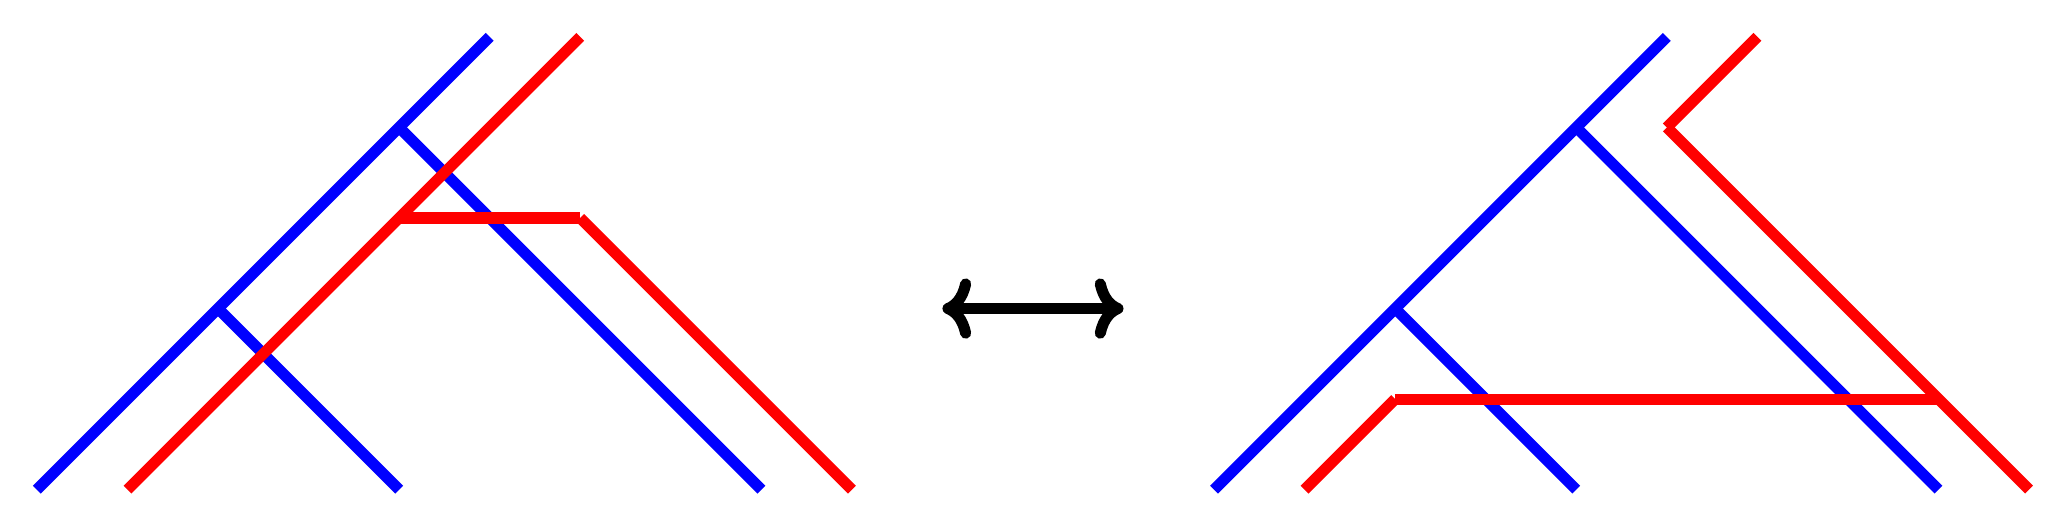
\begin{tikzpicture}[scale=2.3, line width=4pt]
                    \begin{scope}[shift={(0,0)}]
                		\node (0) at (0, 0) {};
                		\node (1) at (2.5, 2.5) {};
                		\node (2) at (1, 1) {};
                		\node (3) at (2, 2) {};
                		\node (4) at (2, 0) {};
                		\node (5) at (4, 0) {};
                		\node (6) at (0.5, 0) {};
                		\node (7) at (3, 2.5) {};
                		\node (8) at (3, 1.5) {};
                		\node (9) at (4.5, 0) {};
                		\node (10) at (2, 1.5) {};
                		\draw[blue] (0.center) to (1.center);
                		\draw[blue] (2.center) to (4.center);
                		\draw[blue] (3.center) to (5.center);
                		\draw[red] (6.center) to (7.center);
                		\draw[red] (10.center) to (8.center);
                		\draw[red] (8.center) to (9.center);
                    \end{scope}

                    \draw[<->] (5,1) to (6,1);

                    \begin{scope}[shift={(6.5,0)}]
                		\node (0) at (0, 0) {};
                		\node (1) at (2.5, 2.5) {};
                		\node (2) at (1, 1) {};
                		\node (3) at (2, 2) {};
                		\node (4) at (2, 0) {};
                		\node (5) at (4, 0) {};
                		\node (6) at (2.5, 2) {};
                		\node (7) at (3, 2.5) {};
                		\node (8) at (4, 0.5) {};
                		\node (9) at (4.5, 0) {};
                		\node (10) at (1, 0.5) {};
                		\node (11) at (0.5, 0) {};
                		\draw[blue] (0.center) to (1.center);
                		\draw[blue] (2.center) to (4.center);
                		\draw[blue] (3.center) to (5.center);
                		\draw[red] (6.center) to (7.center);
                		\draw[red] (10.center) to (8.center);
                		\draw[red] (6.center) to (9.center);
                		\draw[red] (10.center) to (11.center);
                    \end{scope}
                \end{tikzpicture}
            }

            \vspace{-96pt}

            \innerblock{Cospeciation Operator}{
                Makes a guest cospeciate (or not) with its host.

                \centering
                \begin{tikzpicture}[scale=2.3, line width=4pt]
                    \begin{scope}[shift={(0,0)}]
                		\node (0) at (0, 0) {};
                		\node (1) at (2.5, 2.5) {};
                		\node (2) at (1, 1) {};
                		\node (3) at (2, 2) {};
                		\node (4) at (2, 0) {};
                		\node (5) at (4, 0) {};
                		\node (6) at (0.5, 0) {};
                		\node (7) at (3, 2.5) {};
                		\node (8) at (3, 1.5) {};
                		\node (9) at (4.5, 0) {};
                		\node (10) at (2, 1.5) {};
                		\draw[blue] (0.center) to (1.center);
                		\draw[blue] (2.center) to (4.center);
                		\draw[blue] (3.center) to (5.center);
                		\draw[red] (6.center) to (7.center);
                		\draw[red] (8.center) to (10.center);
                		\draw[red] (8.center) to (9.center);
                    \end{scope}

                    \draw[<->] (5,1) to (6,1);

                    \begin{scope}[shift={(6.5,0)}]
                		\node (0) at (0, 0) {};
                		\node (1) at (2.5, 2.5) {};
                		\node (2) at (1, 1) {};
                		\node (3) at (2, 2) {};
                		\node (4) at (2, 0) {};
                		\node (5) at (4, 0) {};
                		\node (6) at (0.5, 0) {};
                		\node (7) at (3, 2.5) {};
                		\node (8) at (3.5, 1) {};
                		\node (9) at (4.5, 0) {};
                		\node (10) at (1.5, 1) {};
                		\draw[blue] (0.center) to (1.center);
                		\draw[blue] (2.center) to (4.center);
                		\draw[blue] (3.center) to (5.center);
                		\draw[red] (6.center) to (7.center);
                        \draw[innerblockbodybgcolor,center*-] (10.center) to (8.center);
                		\draw[red,centero-] (10.center) to (8.center);
                		\draw[red] (8.center) to (9.center);
                    \end{scope}
                \end{tikzpicture}
            }
        }

        \block{Future Work}{
            \begin{itemize}
                \item \textbf{Finish and validate implementation} as an add-on for BEAST
                \item Apply implementation to \textbf{inference on real datasets}
                \item Allow for \textbf{uncertainty in the evolution of the host}
                \item Develop a more sophisticated model; e.g., consider \textbf{preferential host-switching}
                \item \textbf{Utilise geographical information} by constraining a guest and its host to be co-located
            \end{itemize}
        }

        \block{Acknowledgements}{
            \flushleft
            \begin{itemize}
                \item Members of the Computational Evolution Groups at The University of Auckland and ETH~Z\"urich, especially Gabriel Leventhal, David Rasmussen, and Tanja Stadler
            \end{itemize}
        }

        \block{References}{
            \flushleft
            C Andrieu et al. \emph{J. R. Statist. Soc.} B 72.3 (2010). {\normalsize \texttt{\doi{10.1111/j.1467-9868.2009.00736.x}}} \\
            J Sj\"ostrand et al. \emph{Syst. Biol.} 63.3 (2014). \texttt{\doi{10.1093/sysbio/syu007}} \\
            GJ Sz\"oll\H{o}si et al. \emph{Syst. Biol.} 62.3 (2013) \texttt{\doi{10.1093/sysbio/syt003}}
        }

    \end{columns}

\end{document}